\begin{figure}
	\centering
	\begin{minipage}[t]{.4\textwidth}
		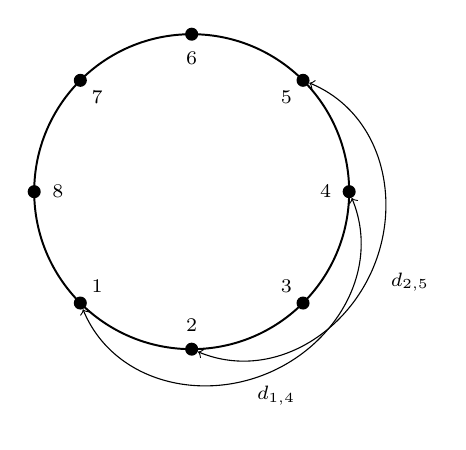
\begin{tikzpicture}[font=\scriptsize, node/.style={circle,thick,draw},
		l_2/.style={line width =0.25mm},
		scale=1, transform shape]
		% equidistant points and arc
		\foreach \x [count=\p] in {0,...,7} {
			\node[shape=circle,fill=black, scale=0.5] (\p) at (\x*45-135:2) {};
		};
		\foreach \x [count=\p] in {0,...,7} {
			\draw (225 + \x*45:1.7) node {\p};
			%				\draw (-30-\x*60:2.4) node {$\bar{\p}$};
		}; 
		\draw[l_2] (4) arc (0:360:2);
		\node (a) at (-22.5:3) {$d_{2, 5}$};
		\draw[<->] (2)  to [out=-22.5,in=-112.5] (-22.5:2.5) to [out=67.5,in=-22.5](5);
		\node (b) at (-67.5:2.8) {$d_{1, 4}$};
		\draw[<->] (1)  to [out=-67.5,in=-157.5] (-67.5:2.5) to [out=22.5,in=-67.5] (4);
		
		\node (bottom) at (0, -2.8) {};
		%		\draw[dashed] (1) -- (3) -- (5) -- (1);
		% axes
		%		\draw [dotted, gray] (-2.6,0) -- (2.6,0);
		%		\draw [dotted, gray] (0,-2.15) -- (0,2.15);
		\end{tikzpicture}
		\subcaption{$d_{1, 4}$ and $d_{2, 5}$ are crossing.}
	\end{minipage}
	\hspace{1cm}
	\begin{minipage}[t]{.4\textwidth}
		\begin{tikzpicture}[font=\scriptsize, node/.style={circle,thick,draw},
		l1_green/.style={thick, green!80!black},
		l1_red/.style={thick, blue!80!white},
		l_2/.style={},
		l_3/.style={line width =0.25mm},
		scale=1, transform shape]
		\draw[l_3] (2, 0) arc (0:360:2);
		
		\draw[l1_green] (5) arc (45:90:2);
		\draw[l1_green] (8) arc (180:270:2);
		\draw[l1_red] (4) arc (0:45:2);
		% equidistant points
		\foreach \x [count=\p] in {0,...,7} {
			\node[shape=circle,fill=black, scale=0.5] (\p) at (\x*45-135:2) {};
		};
		% labels
		\foreach \x [count=\p] in {0,...,7} {
			\draw (225 + \x*45:1.7) node {\p};
			%				\draw (-30-\x*60:2.4) node {$\bar{\p}$};
		};
		
		\node (a) at (10:2.9) {$d_{2, 5}$};
		\draw[l_2, <->] (2)  to [out=-22.5,in=-112.5] (-22.5:2.8) to [out=67.5,in=-22.5](5);
		
		\node (b) at (-15:2.46) {$d_{2, 4}$};
		\draw[l_2,<->] (2)  to [out=-15,in=-135] (-45:2.25) to [out=45,in=-75] (4);
		
		\node (c) at (135:2.7) {$d_{6, 8}$};
		\draw[l_2, <->] (6)  to [out=157.5,in=45] (135:2.4) to [out=-135,in=112.5] (8);
		
		\node (bottom) at (0, -2.8) {};
		%		\draw[dashed] (1) -- (3) -- (5) -- (1);
		% axes
		%		\draw [dotted, gray] (-2.6,0) -- (2.6,0);
		%		\draw [dotted, gray] (0,-2.15) -- (0,2.15);
		\end{tikzpicture}
		\subcaption{$d_{2,4}$, $d_{2, 5}$ and $d_{6, 8}$ are parallel.}
	\end{minipage}
	\caption{Examples of crossing and parallel demands.
		In (b), the green edges lie in between $d_{2, 5}$ and $d_{2, 8}$.
		The blue edge is the only edge in between $d_{2, 4}$ and $d_{2, 5}$.}
	\label{fig:parallel-demands}
\end{figure}